\section{Durchführung}
\label{sec:Durchführung}
Für diesen Versuch wird ein Aufbau verwendet, der in \autoref{fig:Aufbau} zu sehen ist.
\begin{figure}[H]
    \centering
    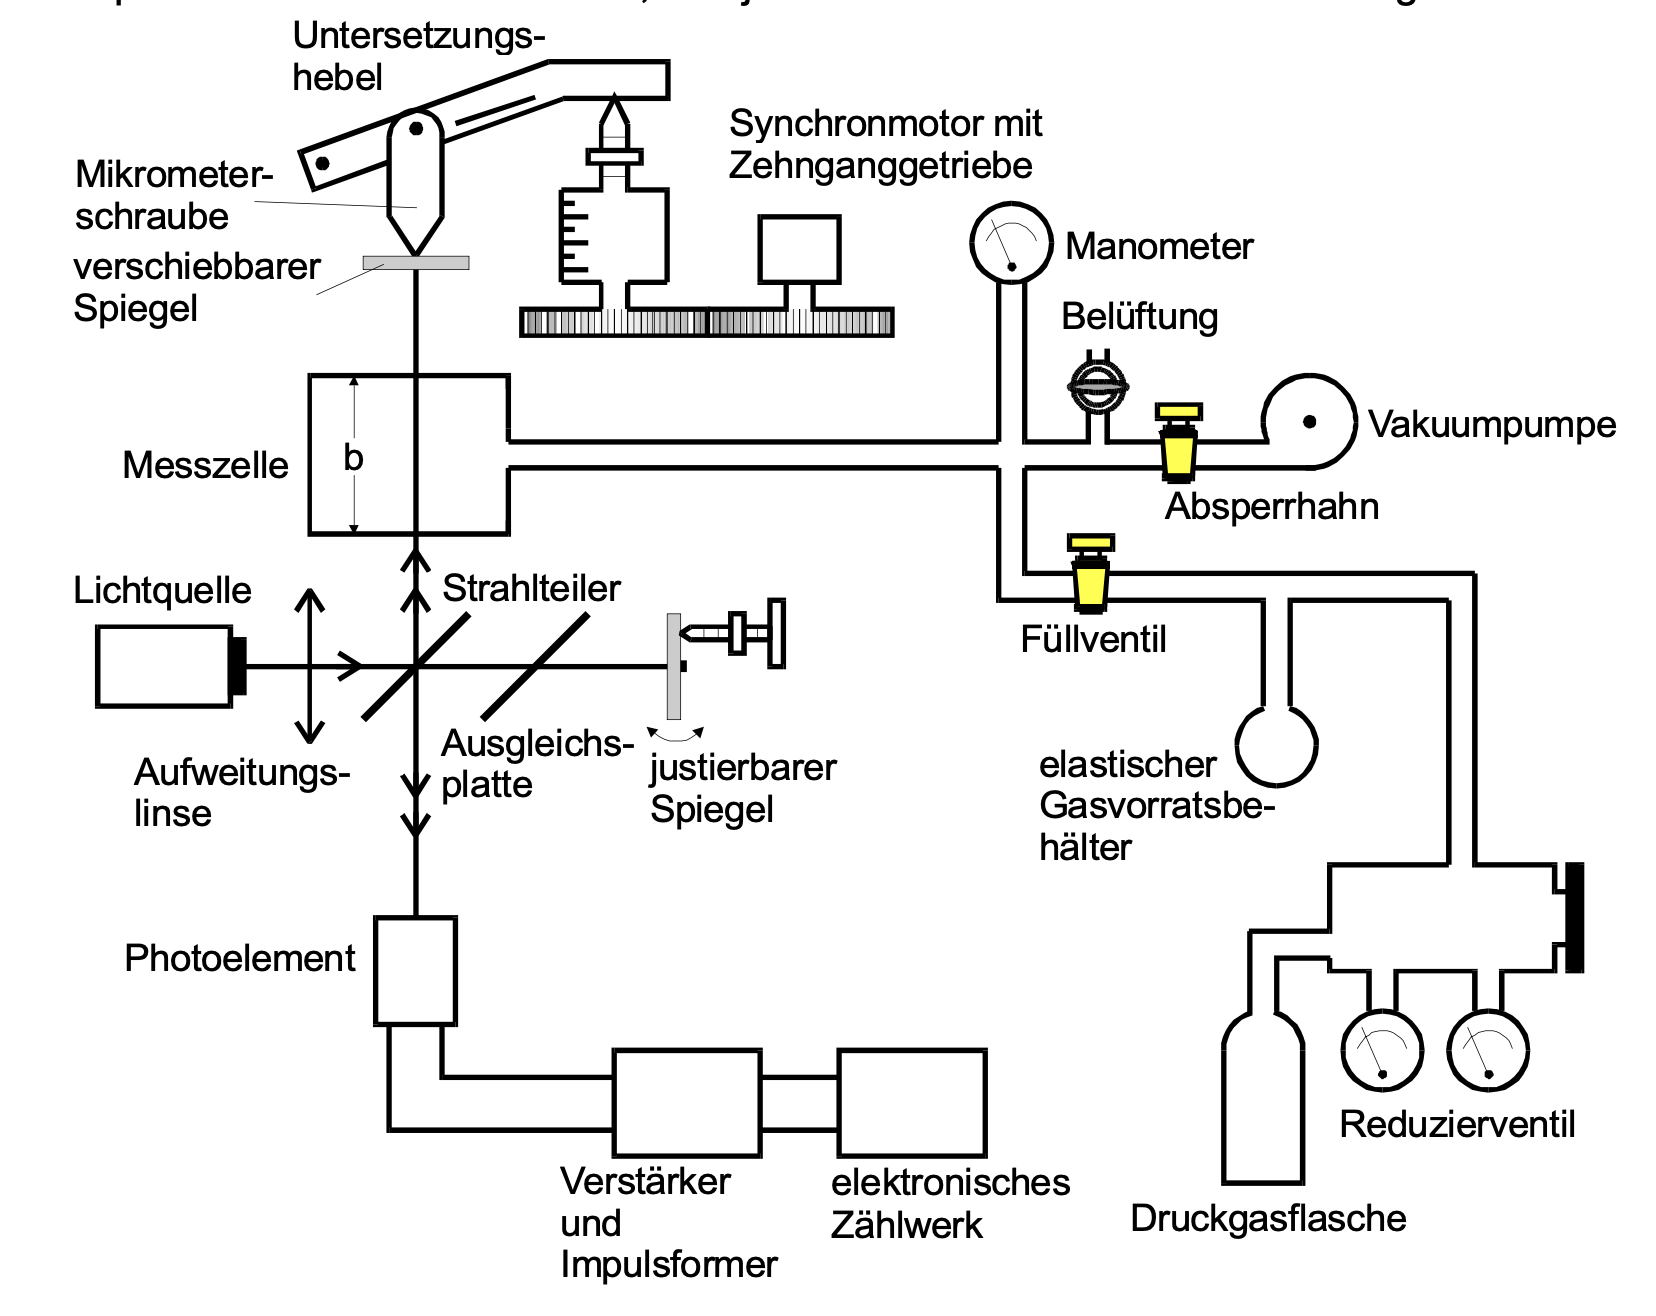
\includegraphics[height=7cm]{content/pics/Aufbau.png}
    \caption{Skizze des Versuchaufbaus \cite{v401}.}
    \label{fig:Aufbau}
  \end{figure}
Bevor die eigentlichen Messungen starten, wird mithilfe der Stellschrauben am justierbaren Spiegel die Überlagerung
der Strahlen so eingestellt, dass diese möglichst exakt übereinander liegen und die Intersitätsextrema breit sind.

Die Photodiode registriert die Maxima und Minima des Interferenzbildes und ein elektronisches Zählwerk zählt diese.

\subsection{Messung der Wellenlänge des Lasers}
Damit die Wellenlänge des Lasers bestimmt werden kann, wird die Mikrometerstellschraube über einen den Synchronmotor in
einem Bereich von $\qty{5}{\milli\metre}$ bis $\qty{10}{\milli\metre}$ in angemessener Geschwindigkeit gedreht. Die 
tatsächliche Änderung der Armlänge ist jedoch um das Übersetzungsverhältnis $u = 1:5,017$ verschieden.

Insgesamt wird dies zehnmal wiederholt, wobei auch das Zurückdrehen der Schraube als Messvorgang verwendet wird.

\subsection{Messung des Brechungsindex von Luft}
Der Brechungsindex von Luft lässt sich bestimmen, indem eine Kammer in dem Strahlengang evakuiert wird. Wärend der Evakuierung
registriert die Photodiode erneut die Maxima und Minima.
Nachdem ein Druck $p'$ erreicht ist, wird ein Belüftungsventil geöffnet und der Druck steigt wieder auf den ursprünglichen 
Druck~$p$ an, während abermals die Maxima und Minima gezählt werden.

Dies wird dreimal druchgeführt, sodass sich hier 6 Messdaten ergeben.